% --- [ Recovery of Post-test Loops ] ------------------------------------------

\subsection{Recovery of Post-test Loops}
\label{sec:recovery_of_post_test_loops}

The control flow recovery results of the Hammock method, the Interval method, and for comparison the theoretical optimum when recovering \textit{post-test loops} (e.g. \texttt{do-while}-loops) from the combined test programs of Coreutils and SQLite are presented in figure \ref{fig:total_results_post_loop}.

The \textbf{Hammock method} correctly recovered $4.65\%$ of the post-test loops present in the test programs (\textit{true positives}). On average, for every $10$ post-test loops of the original source code, the Hammock method recovered $4.1$ post-test loops that were \textit{not} present of the original source code (\textit{false positives}).

The \textbf{Interval method} correctly recovered $62.77\%$ of the post-test loops present in the test programs (\textit{true positives}). On average, for every $10$ post-test loops of the original source code, the Interval method recovered $18.7$ post-test loops that were \textit{not} present of the original source code (\textit{false positives}).

\begin{figure}[htbp]
	\centering
	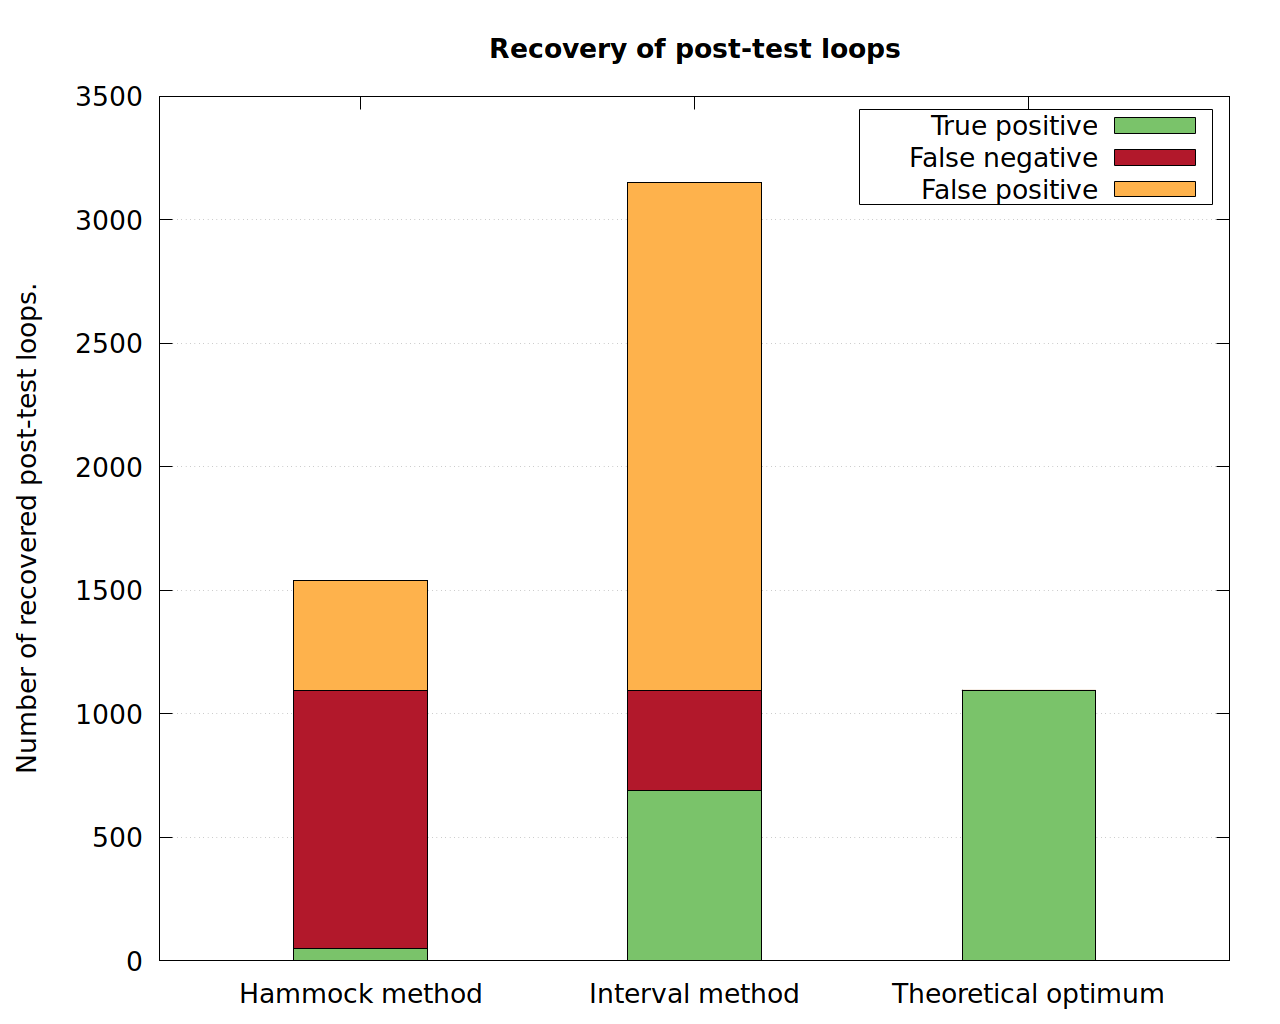
\includegraphics[width=\textwidth]{inc/5_results/results_post_loop.png}
	\caption{Comparison of control flow recovery results for each method when recovering \textit{post-test loops}. The data is based on the combined test programs of Coreutils and SQLite.}
	\label{fig:total_results_post_loop}
\end{figure}
